\chapter{Numerical Experiments}\label{chap: experiments}

In the previous sections, we derived general framework for classification at the top and showed that multiple well-known formulations fall into it. The summary of all formulations presented in this work is in Table~\ref{tab: summary formulations}. The goal of this chapter is to experimentally verify the properties of these formulations. 

\section{Settings}

In this section we describe in detail all settings used for experiments. Formulations from Table~\ref{tab: summary formulations} can be divided into three categories:
\begin{itemize}
  \item The first category contains \TopPush and \TopPushK formulations. Formulations from this category minimize the surrogate approximation of the false-negative rate. As a threshold, these formulations use the mean of a small fraction of the negative samples with the highest scores.
  \item The first category consists of \Grill, \TopMeanK, and \PatMat. These formulations again use the surrogate approximation of the false-negative rate as an objective function. The only exception is the \Grill formulation which also adds the surrogate approximation of the false-positive rate into the objective function for better stability. All three formulation uses some kind of approximation of the top $\tau$-quantile of all scores as a threshold.
  \item The last category consists of \GrillNP, \tauFPL, and \PatMatNP. These formulations use the same objectives as their corresponding formulations from the previous category and differ only in the definition of the decision threshold. All three formulation uses some kind of approximation of the top $\tau$-quantile of negative scores as a threshold.
\end{itemize}
To simplify the setup of all experiments, we decided to test only formulations that use only negative samples for the threshold computation, i.e. only formulations from the first and third categories. The performance of these formulations can be easily compared using some basic performance metrics as we show later in this section.

\subsection{Formulations and Hyperparameters}

At the beginning of this section, we discussed which formulations we use for experiments. In total, we use five different formulations from Table~\ref{tab: summary formulations}, namely \TopPush, \TopPushK, \GrillNP, \tauFPL, and \PatMatNP. Moreover, for \TopPushK we use two different values of~$K = \{5, 10\}$ and consider the resulting formulations as separate formulations, i.e. we have \TopPushK(5) and \TopPushK(10). Similarly, for \GrillNP, \tauFPL and \PatMat we use two different values of~$\tau = \{0.01, 0.05\}.$ For all formulations, we use the hinge loss defined in Notation~\ref{not: surrogates} as a surrogate function.

We have a total of 9 different formulations, however, all these formulations fall into our general framework. To show that these formulations work properly, we have to compare them to some standard methods. In previous chapters, we showed how to solve presented formulations in their primal (Chapters~\ref{chap: linear} and~\ref{chap: deep}) and dual form (Chapter~\ref{chap: dual}). Whenever we use the primal form in the experiments, we use binary cross-entropy defined in the following way as a baseline formulation 
\begin{mini}{\bm{w}}{
  \frac{1}{\nall} \sum_{i \in \I} \Brac{- y_i \log(s_i) - (1 - y_i) \log (1 - s_i)}
  }{\label{eq: crossentropy}}{}
  \addConstraint{s_i}{= f(\bm{x}_i; \bm{w}), \quad i \in \I.}
\end{mini}
We decided to use binary cross-entropy, since it is one of the most used objective functions for binary classification in machine learning applications. In the following text, we will denote binary cross-entropy as \BaseLine for simplicity. In experiments with dual forms, we use C-SVC variant of SVM~\cite{boser1992training, cortes1995support} defined as follows
\begin{mini}{\bm{w}, b, \bm{\xi}}{
  \frac{1}{2} \norm{\bm{w}}^2 + C \sum_{i \in \I} \xi_i
  }{\label{eq: SVM}}{}
  \addConstraint{y_i}{\Brac{\bm{w}^{\top} \phi(\bm{x}_i) + b} \geq 1 - \xi_i, \quad i \in \I}
  \addConstraint{\xi_i}{\geq 0, \quad i \in \I,}
\end{mini}
where~$y_i \in \{-1, 1\}$ for all~$i \in \I$ and~$\phi(\bm{x}_i)$ maps~$\bm{x}_i$ into a higher-dimensional space (see Section~\ref{sec: kernels}). The corresponding dual form is as follows
\begin{maxi}{\bm{\alpha}}{
  - \frac{1}{2} \bm{\alpha}^{\top} \K \bm{\alpha} - \sum_{i = 1}^{\nall} \alpha_i
  }{\label{eq: SVM dual}}{}
  \addConstraint{\sum_{i = 1}^{\nall} y_i \alpha_i}{= 0}
  \addConstraint{0 \leq \alpha_i }{\leq C, \quad i = 1, 2, \ldots, \nall,}
\end{maxi}
where the kernel matrix~$\K$ is defined as
\begin{equation*}
  \K_{i,j} = y_i y_j k(\bm{x}_i, \bm{x}_j) = \phi(\bm{x}_i)^{\top} \phi(\bm{x}_j),
\end{equation*}
for all~$i, j = 1, 2, \ldots, \nall.$ Note that the dual form of C-SVC is very similar to the dual forms of our formulations derived in Chapter~\ref{chap: dual}. In the following text, we will C-SVC as \SVM for simplicity.

In total, we used 11 different formulations in the experiments. However, not all formulations are used for all experiments. For example \GrillNP formulations are not used for experiments with dual forms, since the primal problem is not convex and therefore we did not derive the dual form. Moreover, \BaseLine formulation is also not used for experiments with dual forms. On the other hand, \SVM is used only for experiments with dual forms.

Since considered formulations differ in the number of available hyper-parameters, we decided to fix the number of hyper-parameters per formulation to six. For most of the considered formulations, the remaining hyper-parameter is the regularization constant~$\lambda$. The only exceptions are the formulations derived from \PatMatNP, since they also have the scaling parameter~$\vartheta.$ Therefore, we use the following six values of this hyper-parameter
\begin{equation*}
  \lambda \in \Brac[c]{10^{-5}, 10^{-4}, 10^{-3}, 10^{-2}, 10^{-1}, 1}
\end{equation*}
for all formulations except \PatMatNP. Since we used a slightly different (but equivalent) primal formulation for the derivation of the dual forms, we use~$\lambda$ to compute hyper-parameter~$C$ used in dual forms
\begin{equation*}
  C = \frac{1}{\lambda \ntil},
\end{equation*}
where~$\ntil = \nall$ for \SVM and~$\ntil = \npos$ otherwise. For formulations derived from \PatMatNP, we fixed~$\lambda$ to~$10^{-3}$ and use the following six different values of the scaling parameter
\begin{equation*}
  \vartheta \in \Brac[c]{10^{-5}, 10^{-4}, 10^{-3}, 10^{-2}, 10^{-1}, 1}.
\end{equation*}
In all experiments, the best hyperparameter is selected based on the validation data and the appropriate performance metric.

\subsection{Performance Criteria}

\subsection{Datasets Description}

For the numerical experiments, we consider variety of different datasets summarized in Table~\ref{tab: datasets summary}, that can be divided into three categories:

\paragraph*{Visual recognition datasets:}

This category contains six well-known visual recognition datasets. MNIST \cite{deng2012mnist} and FashionMNIST \cite{xiao2017fashionmnist} are grayscale datasets of digits and fashion items, respectively. CIFAR100~\cite{krizhevsky2009learning} is a dataset of coloured images of different items grouped into 100 classes. CIFAR10 and CIFAR20 merge these classes into 10 and 20 superclasses, respectively. Finally, SVHN2~\cite{netzer2011reading} contains coloured images of house numbers. All datasets from this category are publicly available.

\paragraph*{Steganography datasets:}

For all experiments, we generate dataset from base database of cover images that contains approximately 4 500 000 images from Flickr. All images are JPEG with quality factor 80. To create datasets, we use different techniques of generating stego images. Since generating stego images is expensive, we only generate stego images from 10\% of cover images. Since the database of all images is large, we currently use only a subset with 452 317 cover images and 45 236 stego images.

We generate dataset in the following two ways:
\begin{itemize}
  \item \textbf{Nsf5:} Stego images were generated using simulated F5 with matrix embedding turned off. All images were described using 22500 features and split into train / validation / test set in ratio 0.45 / 0.05 / 0.5.
  \item  \textbf{JMiPOD:} We first select all images that can be cropped to to size $256 \times 256 \times 3$ and than cropped them looselesly using \emph{jpegtran} library. Than, we use J-MiPOD~\cite{cogranne2020steganography} algorithm to generate stego images. We split the data into train / validation / test set in ratio 0.375 / 0.125 / 0.5.
\end{itemize}

Since we are interested in low false-positive rates, we need a lot of negative (cover) samples to estimate it. This is evident in~\eqref{eq: patmat np} where the threshold~$t$ is a surrogate approximation of false-positive rate, i.e., the threshold is computed only from negative samples. Positive samples occurs only in the objective function. Since generating of stego images is expensive and we do not need them to estimate false-positive rate, we decided to reduce the number of positive samples in train data. We use the following three scenarios:
\begin{enumerate}
  \item \textbf{Nsf5-10:} The ratio of stego to cover images is 10\%.
  \item \textbf{Nsf5-1:} The ratio of stego to cover images is 1\%.
  \item \textbf{JMiPOD-10:} The ratio of stego to cover images is 10\%.
\end{enumerate}
The validation and test set is always the same, see Table\ref{tab: Nsf5 dataset}

\paragraph*{Malware detection dataset:}

A renowned cybersecurity company provided malware analysis reports of executable files. This is an extremely tough dataset as individual samples are JSON files whose size ranges from 1kB to 2.5MB. Its structure is highly complicated because each sample has a different number of features, and features may have a complicated structure, such as a list of ports to which the file connects. This is in sharp contrast with standard datasets, where each sample has the same number of features, and each feature is a real number.

All visual recognition datasets from Table~\ref{tab: datasets summary} are originally divided into training and test sets. For these datasets, we select 25\% samples from the training set to obtain the validation set. The rest of the datasets contain only the training set. For these datasets, we select 12.5\% of the samples from the training set as the validation set and 50\% of the samples from the training set as the test set. In all cases, we performed stratified sampling, i.e. we split each class of the data set independently according to the criteria described above.


\begin{table}[!ht]
  \centering
  \resizebox{\columnwidth}{!}{%
    \begin{NiceTabular}{lccrrrrrr}
      \CodeBefore
      \rowcolor{\headercol}{1-2}
      \rowcolors{4}{\rowcol}{}[restart]
      \Body
      \toprule
      \Block[c]{2-1}{\textbf{Dataset}}
      & \Block[c]{2-1}{$y^+$}
      & \Block[c]{2-1}{$d$}
      & \Block[c]{1-2}{\textbf{Train}}
      && \Block[c]{1-2}{\textbf{Validation}}
      && \Block[c]{1-2}{\textbf{Test}} \\
      \cline{4-9}
      &&& \Block[c]{1-1}{$n$}
      & \Block[c]{1-1}{$\frac{\npos}{n}$}
      & \Block[c]{1-1}{$n$}
      & \Block[c]{1-1}{$\frac{\npos}{n}$}
      & \Block[c]{1-1}{$n$}
      & \Block[c]{1-1}{$\frac{\npos}{n}$} \\
      \midrule
      MNIST
      & 1
      & $28 \times 28 \times 1$
      & 45 000
      & 11.3\%
      & 15 000
      & 11.2\%
      & 10 000
      & 11.4\% \\
      FashionMNIST
      & 1
      & $28 \times 28\times 1$
      & 45 000
      & 10.0\%
      & 15 000
      & 9.9\%
      & 10 000
      & 10.0\% \\
      CIFAR10
      & 1
      & $32 \times 32 \times 3$
      & 37 500
      & 10.0\%
      & 12 500
      & 9.9\%
      & 10 000
      & 10.0\% \\
      CIFAR20
      & 1
      & $32 \times 32 \times 3$
      & 37 500
      & 5.0\%
      & 12 500
      & 5.1\%
      & 10 000
      & 5.0\% \\
      CIFAR100
      & 1
      & $32 \times 32 \times 3$
      & 37 500
      & 1.0\%
      & 12 500
      & 1.0\%
      & 10 000
      & 1.0\% \\
      SVHN2
      & 1
      & $32 \times 32\times 3$
      & 54 944
      & 18.9\%
      & 18 313
      & 18.9\%
      & 26 032
      & 19.6\% \\
      SVHN2-Extra
      & 1
      & $32 \times 32\times 3$
      & 453 291
      & 17.3\%
      & 151 097
      & 17.1\%
      & 26 032
      & 19.6\% \\
      \midrule
      Nsf5 Small
      & ---
      & $22 510 \times 1$
      & 186 583
      & 9.1\%
      & 62 194
      & 9.1\%
      & 248 776
      & 9.1\% \\
      JMiPOD Small
      & ---
      & $256 \times 256\times 3$
      & 186 515
      & 9.1\%
      & 62 172
      & 9.1\%
      & 248 686
      & 9.1\% \\
      \midrule
      Malware
      & ---
      & variable
      & 6 580 166
      & 87.22\%
      & ---
      & ---
      & 800 346
      & 91.8\% \\
      \bottomrule
    \end{NiceTabular}
  }
  \caption{Structure of the used datasets: The training, validation and testing sets show the positive label~$y^+,$ the number of features~$d$, samples~$n$ and the fraction of positive samples~$\frac{\npos}{n}$.}
  \label{tab: datasets summary}
\end{table}

\section{Results}

\subsection{Linear Model and Full Data}

\subsection{Linear Model and SGD}

% \begin{figure}[!ht]
%   \centering
%   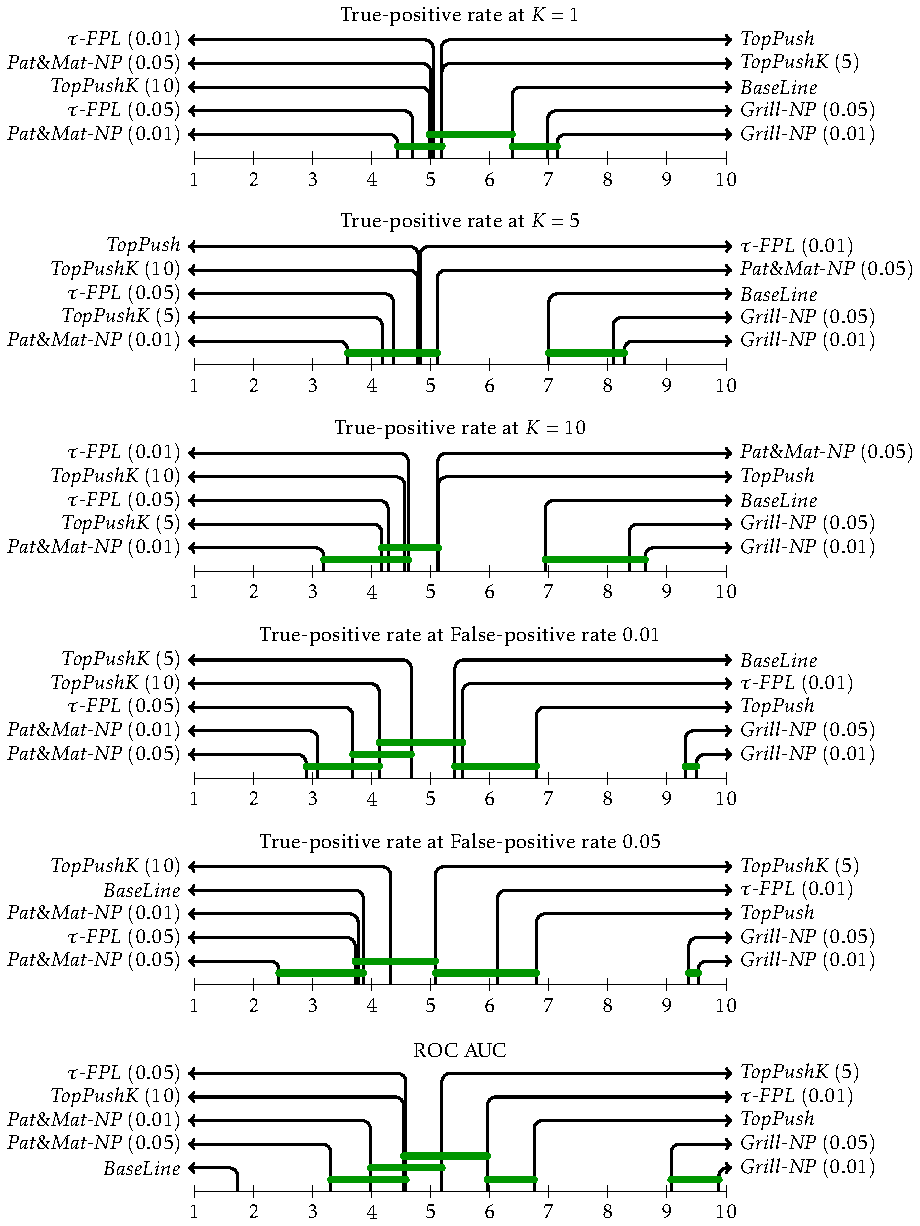
\includegraphics[width = \linewidth]{images/critical_diagrams_primal.pdf}
%   \caption{Critical difference (CD) diagrams (level of importance 0.05) of the Nemenyi post hoc test for the Friedman test. Each diagram shows the mean rank of each method, with rank 1 being the best. Black wide horizontal lines group together methods with the mean ranks that are not significantly different. The critical difference diagrams were computed for mean rank averages over all datasets of the tpr@fpr at $\tau=0.05$ (top) and at $\tau=0.01$ (bottom).}
%   \label{fig: critical diagrams primal}
% \end{figure}

% \subsection{Dual Formulations}

% \begin{figure}[!ht]
%   \centering
%   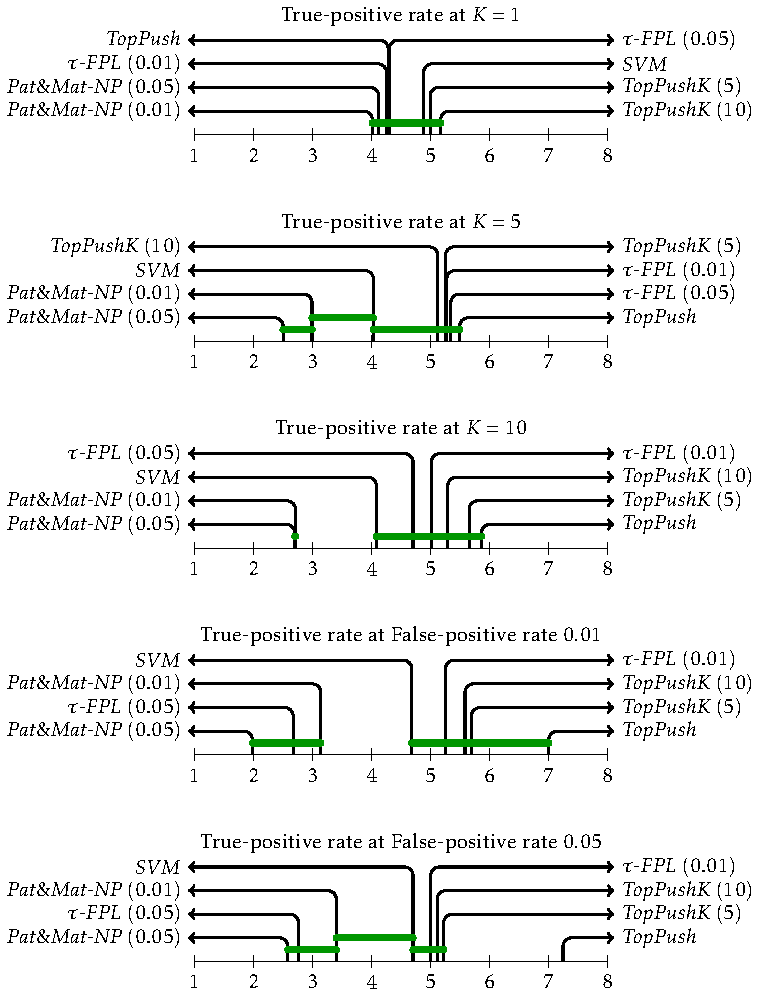
\includegraphics[width = \linewidth]{images/critical_diagrams_dual_linear.pdf}
%   \caption{Critical difference (CD) diagrams (level of importance 0.05) of the Nemenyi post hoc test for the Friedman test. Each diagram shows the mean rank of each method, with rank 1 being the best. Black wide horizontal lines group together methods with the mean ranks that are not significantly different. The critical difference diagrams were computed for mean rank averages over all datasets of the tpr@fpr at $\tau=0.05$ (top) and at $\tau=0.01$ (bottom).}
%   \label{fig: critical diagrams dual linear}
% \end{figure}

% \begin{figure}[!ht]
%   \centering
%   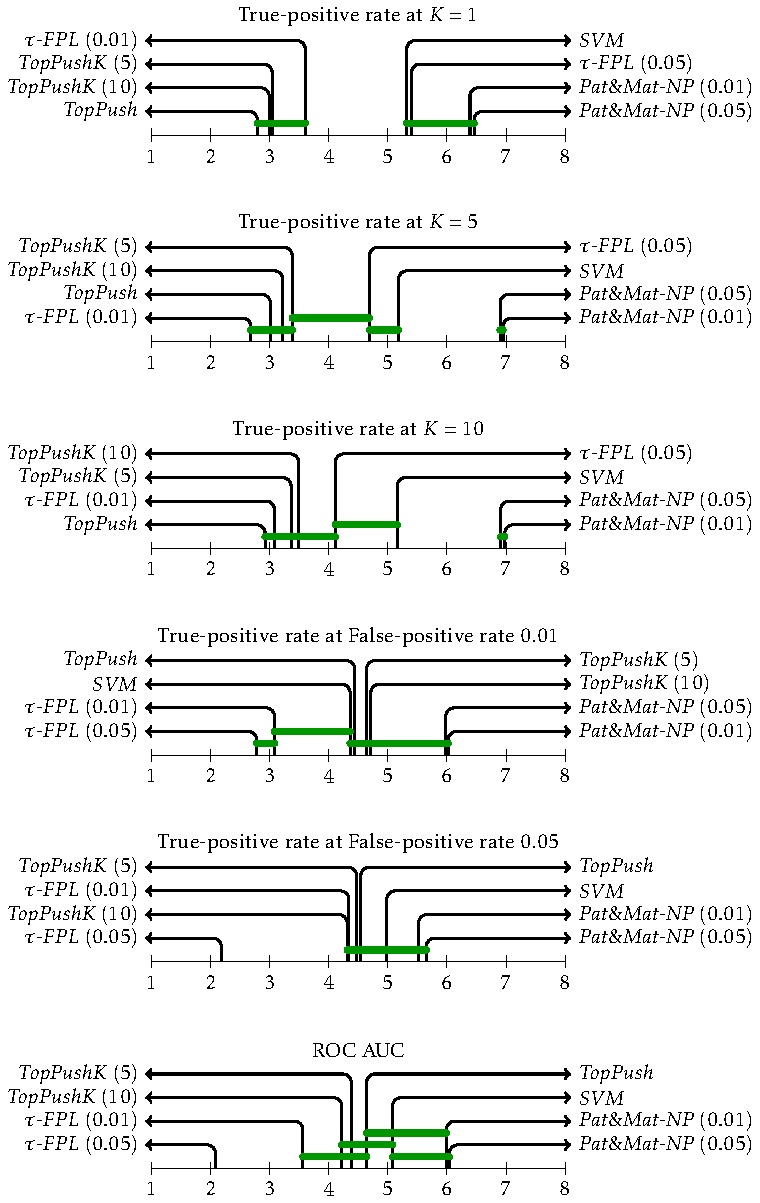
\includegraphics[width = \linewidth]{images/critical_diagrams_dual.pdf}
%   \caption{Critical difference (CD) diagrams (level of importance 0.05) of the Nemenyi post hoc test for the Friedman test. Each diagram shows the mean rank of each method, with rank 1 being the best. Black wide horizontal lines group together methods with the mean ranks that are not significantly different. The critical difference diagrams were computed for mean rank averages over all datasets of the tpr@fpr at $\tau=0.05$ (top) and at $\tau=0.01$ (bottom).}
%   \label{fig: critical diagrams dual}
% \end{figure}

% \subsection{Non-linear model and SGD}

% \begin{figure}[!ht]
%   \centering
%   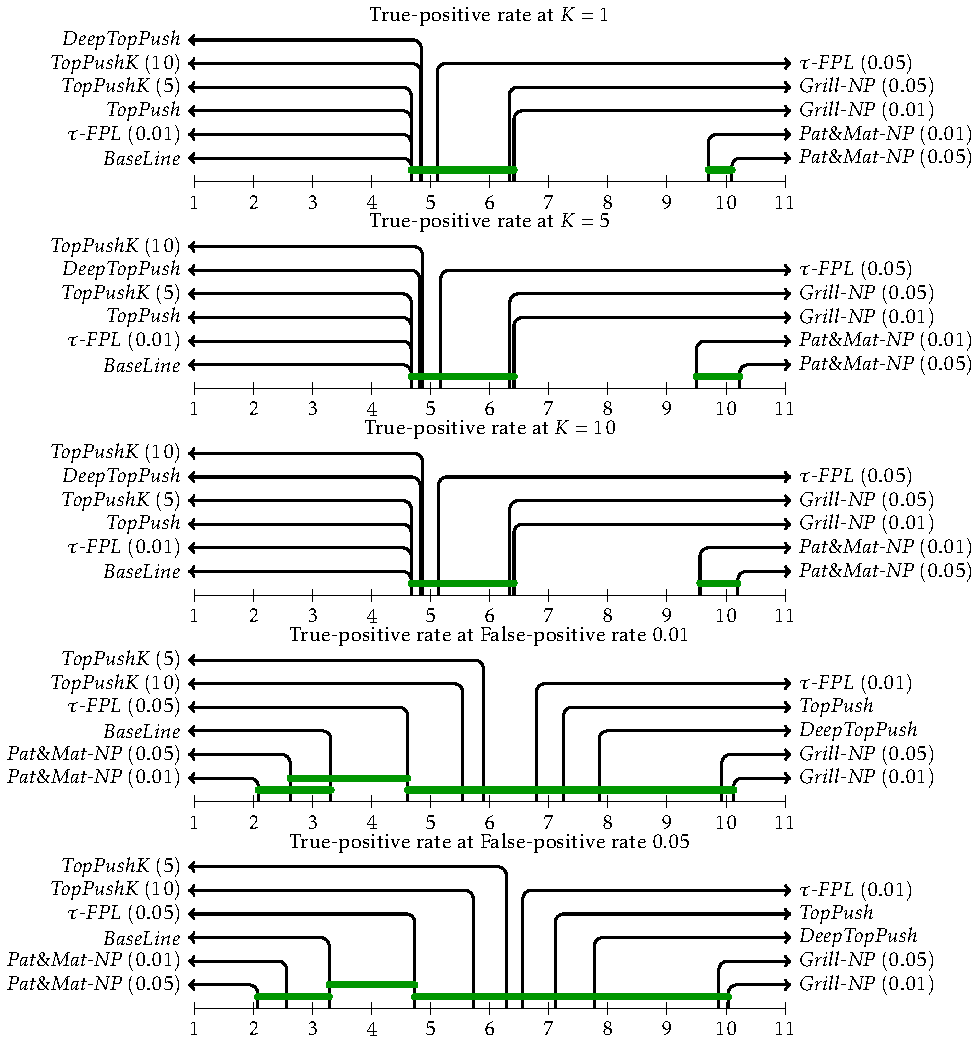
\includegraphics[width = \linewidth]{images/critical_diagrams_primalnn.pdf}
%   \caption{Critical difference (CD) diagrams (level of importance 0.05) of the Nemenyi post hoc test for the Friedman test. Each diagram shows the mean rank of each method, with rank 1 being the best. Black wide horizontal lines group together methods with the mean ranks that are not significantly different. The critical difference diagrams were computed for mean rank averages over all datasets of the tpr@fpr at $\tau=0.05$ (top) and at $\tau=0.01$ (bottom).}
%   \label{fig: critical diagrams primalnn}
% \end{figure}

\section{Conclusion}

\subsection{Linear Model}

In this paper, we achieved the following results:
\begin{itemize}
  \item We presented a unified framework for the three criteria from Chapter~\ref{chap: framework}. These criteria include ranking, accuracy at the top and hypothesis testing.
  \item We showed that several known methods (\TopPush, \Grill, \tauFPL) fall into our framework and derived some completely new methods (\PatMat, \PatMatNP).
  \item We performed a theoretical analysis of the methods. We showed that known methods suffer from certain disadvantages. While \TopPush and \tauFPL are sensitive to outliers, \Grill is non-convex. We proved the global convergence of the stochastic gradient descent for \PatMat and \PatMatNP.
  \item We performed a numerical comparison and we showed a good performance of our method \PatMatNP.
\end{itemize}


\subsection{Dual}\label{sec:Conclusion}

In this paper, we analyzed and extended the general framework for binary classification on top samples from~\cite{adam2021general} to nonlinear problems. Achieved results can be summarized as follows:
\begin{itemize}
  \item We derived the dual formulations for \TopPush, \TopPushK and \PatMat.
  \item We proposed a new method for solving the dual problems. We performed its complexity analysis. For selected surrogate functions we also derived the exact formulas needed in the method.
  \item We performed a numerical analysis of the proposed method. We showed its good convergence as well as improved performance of nonlinear kernels over the linear one.
\end{itemize}
Based on the numerical analysis from Section~\ref{sec:Numerical experiments}, we recommend using \TopPush or \TopPushK for problems where the resulting recall should be small. Otherwise, we recommend using \PatMat with an appropriately selected~$\tau$ parameter.

\subsection{Neural Networks}

We proposed \DeepTopPush as an efficient method for solving the constrained non-decomposable problem of accuracy at the top, which focuses on the performance only above a threshold. We implicitly removed some optimization variables, created an unconstrained end-to-end network and used the stochastic gradient descent to train it. We modified the minibatch so that the sampled threshold (computed on a minibatch) is a good estimate of the true threshold (computed on all samples). We showed both theoretically and numerically that this procedure reduces the bias of the sampled gradient. The time increase over the standard method with no threshold is small. We demonstrated the usefulness of \DeepTopPush both on visual recognition datasets, a ranking problem and on a real-world application of malware detection.
